\documentclass[conference,10pt]{IEEEtran}
\usepackage[T1]{fontenc}
\usepackage{amsmath,amssymb}
\usepackage{graphicx}
\usepackage{booktabs}
\usepackage{xcolor}
\usepackage[hidelinks]{hyperref}
\newcommand{\MainCost}{8.32}
\newcommand{\MainLo}{7.31}
\newcommand{\MainHi}{9.45}
\newcommand{\BestRule}{risk-greedy}
\newcommand{\BestRuleCost}{8.96}
\newcommand{\GainVsRule}{7}
\newcommand{\GainVsRuleAbs}{0.64}
\newcommand{\GainVsRuleLo}{0.17}
\newcommand{\GainVsRuleHi}{1.02}
\newcommand{\FlatCost}{10.21}
\newcommand{\PPOCost}{14.93}
\newcommand{\OracleCost}{7.50}
\newcommand{\LastObsCost}{8.42}
\newcommand{\NoInspCost}{8.19}
\newcommand{\NoDemoCost}{8.16}
\newcommand{\SharedCost}{7.90}
\newcommand{\RuleDemoCost}{9.03}
\newcommand{\PretrainCost}{8.29}
\newcommand{\PlannerCost}{8.61}
\newcommand{\EnsembleCost}{8.12}
\newcommand{\NothingCost}{301}
\newcommand{\RandomCost}{301}
\newcommand{\OracleRuleCost}{8.69}
\newcommand{\VanillaCost}{18.08}
\newcommand{\Funding}{0.44}
\newcommand{\Sufficiency}{0.88}
\newcommand{\UnlimitedCost}{4.99}
\newcommand{\Episodes}{200}
\newcommand{\NPairs}{15,190}
\newcommand{\RoutineSigma}{0.35}
\newcommand{\AgeCoef}{0.63}
\newcommand{\AdtCoef}{-0.74}
\newcommand{\ObservedYears}{59--64}
\newcommand{\ModelYears}{20--21}
\newcommand{\UnmaintainedFactor}{3}
\newcommand{\OODTotal}{6}
\newcommand{\OODWins}{3}
\newcommand{\OODLosses}{1}
\newcommand{\CutSaving}{11.71}
\newcommand{\CutLo}{6.47}
\newcommand{\CutHi}{17.05}
\newcommand{\CutLoss}{\textminus{}11.71}
\newcommand{\CutOurs}{16.97}
\newcommand{\CutRule}{28.7}
\newcommand{\FastSaving}{1.19}
\newcommand{\FastLo}{0.52}
\newcommand{\FastHi}{1.89}
\newcommand{\FastLoss}{\textminus{}1.19}
\newcommand{\FastOurs}{15.64}
\newcommand{\FastRule}{16.83}
\newcommand{\NoisySaving}{\textminus{}0.56}
\newcommand{\NoisyLo}{\textminus{}1.36}
\newcommand{\NoisyHi}{0.21}
\newcommand{\NoisyLoss}{0.56}
\newcommand{\NoisyOurs}{12.99}
\newcommand{\NoisyRule}{12.43}
\newcommand{\SlowSaving}{1.06}
\newcommand{\SlowLo}{0.96}
\newcommand{\SlowHi}{1.17}
\newcommand{\SlowLoss}{\textminus{}1.06}
\newcommand{\SlowOurs}{5.21}
\newcommand{\SlowRule}{6.27}
\newcommand{\UnmodSaving}{0.22}
\newcommand{\UnmodLo}{\textminus{}0.55}
\newcommand{\UnmodHi}{0.93}
\newcommand{\UnmodLoss}{\textminus{}0.22}
\newcommand{\UnmodOurs}{12.88}
\newcommand{\UnmodRule}{13.10}
\newcommand{\UnseenSaving}{\textminus{}3.84}
\newcommand{\UnseenLo}{\textminus{}8.83}
\newcommand{\UnseenHi}{\textminus{}0.42}
\newcommand{\UnseenLoss}{3.84}
\newcommand{\UnseenOurs}{16.97}
\newcommand{\UnseenRule}{13.13}
\newcommand{\EnsembleGain}{9}
\newcommand{\GainVsPlanner}{0.30}
\newcommand{\GainVsPlannerLo}{\textminus{}0.19}
\newcommand{\GainVsPlannerHi}{0.88}
\newcommand{\OracleDiff}{\textminus{}0.82}
\newcommand{\OracleLo}{\textminus{}1.11}
\newcommand{\OracleHi}{\textminus{}0.55}
\newcommand{\OracleGap}{0.82}
\newcommand{\OracleGapLo}{0.55}
\newcommand{\OracleGapHi}{1.11}
\newcommand{\LastObsDiff}{0.10}
\newcommand{\LastObsLo}{\textminus{}0.31}
\newcommand{\LastObsHi}{0.54}
\newcommand{\LastObsGap}{\textminus{}0.10}
\newcommand{\LastObsGapLo}{\textminus{}0.54}
\newcommand{\LastObsGapHi}{0.31}
\newcommand{\NoInspDiff}{\textminus{}0.13}
\newcommand{\NoInspLo}{\textminus{}0.33}
\newcommand{\NoInspHi}{0.08}
\newcommand{\NoInspGap}{0.13}
\newcommand{\NoInspGapLo}{\textminus{}0.08}
\newcommand{\NoInspGapHi}{0.33}
\newcommand{\PretrainDiff}{\textminus{}0.03}
\newcommand{\PretrainLo}{\textminus{}0.21}
\newcommand{\PretrainHi}{0.14}
\newcommand{\PretrainGap}{0.03}
\newcommand{\PretrainGapLo}{\textminus{}0.14}
\newcommand{\PretrainGapHi}{0.21}
\newcommand{\SharedDiff}{\textminus{}0.41}
\newcommand{\SharedLo}{\textminus{}0.81}
\newcommand{\SharedHi}{\textminus{}0.08}
\newcommand{\SharedGap}{0.41}
\newcommand{\SharedGapLo}{0.08}
\newcommand{\SharedGapHi}{0.81}
\newcommand{\EnsembleDiff}{\textminus{}0.20}
\newcommand{\EnsembleLo}{\textminus{}0.36}
\newcommand{\EnsembleHi}{\textminus{}0.09}
\newcommand{\EnsembleGap}{0.20}
\newcommand{\EnsembleGapLo}{0.09}
\newcommand{\EnsembleGapHi}{0.36}
\newcommand{\MainSeedSaveRule}{0.64}
\newcommand{\MainSeedSaveRuleLo}{0.13}
\newcommand{\MainSeedSaveRuleHi}{1.05}
\newcommand{\MainSeedSavePlanner}{0.30}
\newcommand{\MainSeedSavePlannerLo}{\textminus{}0.23}
\newcommand{\MainSeedSavePlannerHi}{0.90}
\newcommand{\PretrainSeedSaveRule}{0.67}
\newcommand{\PretrainSeedSaveRuleLo}{0.14}
\newcommand{\PretrainSeedSaveRuleHi}{1.07}
\newcommand{\PretrainSeedSavePlanner}{0.32}
\newcommand{\PretrainSeedSavePlannerLo}{\textminus{}0.22}
\newcommand{\PretrainSeedSavePlannerHi}{1.02}
\newcommand{\NoDemoSeedSaveRule}{0.80}
\newcommand{\NoDemoSeedSaveRuleLo}{0.23}
\newcommand{\NoDemoSeedSaveRuleHi}{1.27}
\newcommand{\NoDemoSeedSavePlanner}{0.46}
\newcommand{\NoDemoSeedSavePlannerLo}{\textminus{}0.29}
\newcommand{\NoDemoSeedSavePlannerHi}{1.31}
\newcommand{\RuleDemoSeedSaveRule}{\textminus{}0.07}
\newcommand{\RuleDemoSeedSaveRuleLo}{\textminus{}0.26}
\newcommand{\RuleDemoSeedSaveRuleHi}{0.04}
\newcommand{\RuleDemoSeedSavePlanner}{\textminus{}0.42}
\newcommand{\RuleDemoSeedSavePlannerLo}{\textminus{}1.05}
\newcommand{\RuleDemoSeedSavePlannerHi}{0.38}
\newcommand{\SharedSeedSaveRule}{1.05}
\newcommand{\SharedSeedSaveRuleLo}{0.50}
\newcommand{\SharedSeedSaveRuleHi}{1.55}
\newcommand{\SharedSeedSavePlanner}{0.71}
\newcommand{\SharedSeedSavePlannerLo}{0.15}
\newcommand{\SharedSeedSavePlannerHi}{1.41}
\newcommand{\FlatSeedSaveRule}{\textminus{}1.25}
\newcommand{\FlatSeedSaveRuleLo}{\textminus{}3.10}
\newcommand{\FlatSeedSaveRuleHi}{0.22}
\newcommand{\FlatSeedSavePlanner}{\textminus{}1.59}
\newcommand{\FlatSeedSavePlannerLo}{\textminus{}3.34}
\newcommand{\FlatSeedSavePlannerHi}{\textminus{}0.22}
\newcommand{\VanillaSeedSaveRule}{\textminus{}9.13}
\newcommand{\VanillaSeedSaveRuleLo}{\textminus{}12.03}
\newcommand{\VanillaSeedSaveRuleHi}{\textminus{}6.47}
\newcommand{\VanillaSeedSavePlanner}{\textminus{}9.47}
\newcommand{\VanillaSeedSavePlannerLo}{\textminus{}12.22}
\newcommand{\VanillaSeedSavePlannerHi}{\textminus{}7.04}
\newcommand{\OracleSeedSaveRule}{1.46}
\newcommand{\OracleSeedSaveRuleLo}{1.03}
\newcommand{\OracleSeedSaveRuleHi}{1.84}
\newcommand{\OracleSeedSavePlanner}{1.12}
\newcommand{\OracleSeedSavePlannerLo}{0.54}
\newcommand{\OracleSeedSavePlannerHi}{1.85}
\newcommand{\LastObsSeedSaveRule}{0.54}
\newcommand{\LastObsSeedSaveRuleLo}{\textminus{}0.16}
\newcommand{\LastObsSeedSaveRuleHi}{1.13}
\newcommand{\LastObsSeedSavePlanner}{0.20}
\newcommand{\LastObsSeedSavePlannerLo}{\textminus{}0.48}
\newcommand{\LastObsSeedSavePlannerHi}{0.95}
\newcommand{\NoInspSeedSaveRule}{0.77}
\newcommand{\NoInspSeedSaveRuleLo}{0.26}
\newcommand{\NoInspSeedSaveRuleHi}{1.19}
\newcommand{\NoInspSeedSavePlanner}{0.43}
\newcommand{\NoInspSeedSavePlannerLo}{\textminus{}0.12}
\newcommand{\NoInspSeedSavePlannerHi}{1.11}
\newcommand{\PPOSeedSaveRule}{\textminus{}5.97}
\newcommand{\PPOSeedSaveRuleLo}{\textminus{}7.51}
\newcommand{\PPOSeedSaveRuleHi}{\textminus{}4.57}
\newcommand{\PPOSeedSavePlanner}{\textminus{}6.31}
\newcommand{\PPOSeedSavePlannerLo}{\textminus{}7.81}
\newcommand{\PPOSeedSavePlannerHi}{\textminus{}4.94}
\newcommand{\MainInsp}{3.2}
\newcommand{\MainClosed}{5.6}
\newcommand{\RuleClosed}{4.8}
\newcommand{\MainAgency}{2.78}
\newcommand{\RuleAgency}{2.37}
\newcommand{\MainClosure}{1.95}
\newcommand{\RuleClosure}{1.47}
\newcommand{\MainRisk}{3.45}
\newcommand{\RuleRisk}{4.44}
\newcommand{\MainSalvage}{0.13}
\newcommand{\RuleSalvage}{0.68}
\newcommand{\DemoEpisodes}{100}
\newcommand{\PlannerDemoCost}{8.30}
\newcommand{\DQNms}{0.19}
\newcommand{\Plannerms}{347}
\newcommand{\SpeedUp}{1,830}


\newcommand{\repo}{\url{https://github.com/b23bb1023/Bridge-RL-agent}}
\setlength{\textfloatsep}{8pt plus 2pt minus 2pt}
\setlength{\dbltextfloatsep}{8pt plus 2pt minus 2pt}

\begin{document}
\title{BridgePulse-RL: Deep Q-Learning for Budget-Constrained Bridge Inspection and Repair}
\author{\IEEEauthorblockN{K V Raghava}
\IEEEauthorblockA{Code, data, trained agents and results: \repo}}
\maketitle

\begin{figure*}[t]
\centering
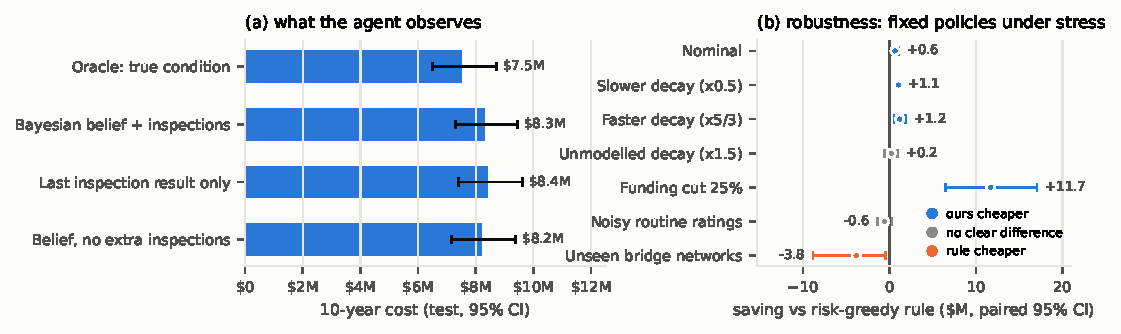
\includegraphics[width=\textwidth]{figures/fig2_information.pdf}
\vspace{-4pt}
\caption{(a) Test cost by what the agent observes (95\% CI). (b) Paired saving of our agent over the best tuned rule when the world differs from training (no retraining; 95\% CI).}
\label{fig:info}
\end{figure*}

\section{Problem and environment}
A road agency must keep ten aging bridges open for ten years ($T{=}120$ months) on half the money it
needs, without seeing their true condition. Each month it issues one work order. The bridges are real
Pennsylvania bridges from the National Bridge Inventory (NBI), with their deck areas, traffic (ADT),
truck shares and detour lengths (3 arterial, 4 collector, 3 local). Funding of \$\Funding M/yr,
half the level at which the best tuned rule gets within 10\% of its unlimited-money cost, accrues
monthly into an account that carries savings forward.

\textbf{Hidden dynamics, fitted to real data.} Bridge $i$ has condition $c_i\in\{0..4\}$ (Excellent to
Critical, from its lowest NBI component rating). Without repair, it drops one state per month with
probability $q_c\exp(\beta_a\frac{\text{age}_i-50}{50}+\beta_w(w_i-\frac12))$, where $w_i$ is log
traffic. The hazards $q_c$, the effects $\beta_a{=}{\AgeCoef}$ and $\beta_w{=}{\AdtCoef}$, the routine rating
noise ($\sigma{=}\RoutineSigma$) and the hidden-state mix are fitted jointly by maximum likelihood. We
use an HMM likelihood over \NPairs{} pairs of 2022/2024 inspections, so that rating noise is not
mistaken for decay. Inventory bridges get upkeep we do not model (\ObservedYears{} years per state),
so the hazards are scaled by \UnmaintainedFactor{} (\ModelYears{} years). An open Critical bridge closes
w.p.\ 0.25 per month until a major repair.

\textbf{Observations and belief.} An inspection reports $o\sim O(o|c)\propto e^{-(o-c)^2/2\sigma^2}$.
Routine inspections are free and happen every 24 months with the fitted $\sigma$. Paid in-depth
inspections ($\sigma{=}0.25$) can be bought any month. The environment keeps the exact posterior
$b_i\in\Delta^4$ of every bridge. It is updated by Bayes' rule for inspections, by the repair and decay
kernels, and by closures: a closure reveals $c_i{=}4$, and staying open is weak evidence against it.
Initial conditions are drawn from the same posterior, so the filter is exact; unit tests check it by
brute-force enumeration.

\textbf{State} $s_t\in[0,1]^{103}$: for each bridge, $b_i$, log closure and repair costs, age, months
since inspection, and a closed flag; plus the account balance, month of year and $t/T$.
\textbf{Actions} ($|\mathcal{A}|{=}31$): defer; inspect bridge $i$; minor repair of $i$ (Good/Fair
improve one state w.p.\ 0.9); major repair of $i$ (to Excellent w.p.\ 0.95, else Good; reopens the
bridge). A mask removes unaffordable work orders, and inspection or minor repair of a closed bridge.
\textbf{Reward} (\$M):
$r_t{=}-[C(a_t)+\sum_i D_iU_i+\sum_i(1{-}D_i)\rho(c_i)R_i+\mathbf{1}[t{=}T]\sum_i S_i(c_i)]$.
$C$ is the agency cost (16/160/1{,}600\,\$/m$^2$ of deck for inspection, minor or major repair). $U_i$
is the monthly road-user cost of a closure ($D_i{=}1$), ADT$\times$detour$\times$vehicle cost.
$\rho{=}[0,.05,.2,.6,1]$ scales a structural-risk cost $R_i$. $S_i$ is the cost to restore the bridge
at the end. The negative return is the true 10-year cost, which we report. In training, the risk and
restore terms are replaced by their belief expectation, which leaves expected returns unchanged and
lowers the variance.

\section{Agent and baselines}
\textbf{Decomposed masked DQN.} A shared encoder embeds each bridge's features with the global ones.
Mean/max pooling gives a network context. From its embedding and the context, bridge $i$ outputs a
baseline $B_i$, values $Q_i^k$ for each work order $k$ on itself, and a shadow price of money
$\lambda_i{\ge}0$. Then $Q(s,a){=}\sum_iQ_i(s,a)$, where $Q_i$ is $B_i$ for defer, $Q_i^k$ for
work on $i$, and $B_i-\lambda_i\,\mathrm{cost}_{kj}$ for work on another bridge $j$, which affects $i$
only through the money it uses. Each $Q_i$ is trained on bridge $i$'s share of the reward, with
targets at the joint greedy next action. The agent uses a masked $\arg\max$ when acting and in the
double-DQN target, 3-step returns, $\gamma{=}0.99$, soft targets ($\tau{=}0.005$), 8 environments and
$3{\times}10^5$ steps. The checkpoint with the best cost on 40 validation episodes is kept.

\textbf{Learning from a planner.} A lookahead planner improves the best tuned rule by simulation. Each
month it shortlists the rule's choice, defer, the four repairs saving the most risk per dollar, and the
most informative inspection. It scores each candidate by 8 rollouts of that work order followed by the
rule to the horizon. Rollouts start from conditions sampled from the belief (stratified per bridge) and
share random numbers. The planner leaves the rule's choice only if the paired saving exceeds one
standard error. We record \DemoEpisodes{} planner episodes and pre-train the DQN on them
with TD plus a large-margin loss $\max_a[Q(s,a){+}0.5\,\mathbf{1}(a{\ne}a_E)]-Q(s,a_E)$. During
Q-learning, a quarter of each batch comes from the demonstrations and the margin fades to zero.

\textbf{Baselines and protocol.} \emph{Rules:} the four in Table~\ref{tab:main}, with thresholds
grid-searched on separate tuning episodes. \emph{Maskable PPO} with $10^6$ steps. \emph{DQN ablations:} rule instead of planner
demonstrations; none; an undecomposed shared network; a flat MLP; vanilla DQN (no masks, dueling,
double estimator or demonstrations). \emph{Information variants:} the agent sees the truth, only the
last inspection, or cannot buy inspections, each warm-started by a planner with the same information.
The main agent and PPO use 5 seeds, the ablations 2. The test uses \Episodes{} held-out episodes on
which every policy faces the same random draws, so differences are paired, with 95\% bootstrap CIs.

\begin{table}[t]
\centering
\caption{Ten-year cost on \Episodes{} test episodes (\$M). CIs (95\%) resample test episodes, holding the trained agents fixed. $\Delta$: paired extra cost over our agent. Closed: bridge-months. Insp.: paid inspections. $^\dagger$sees the true condition.}
\label{tab:main}
\scriptsize
\setlength{\tabcolsep}{2.5pt}
\begin{tabular}{@{}lrrrr@{}}
\toprule
Policy & Cost \$M [95\% CI] & $\Delta$ vs ours & Closed & Insp. \\
\midrule
\textbf{DQN (ours)} & 8.32 [7.31, 9.45] & -- & 6 & 3.2 \\
DQN (ours), 5-seed ensemble & 8.12 [7.12, 9.23] & \textminus{}0.20 & 5 & 0.7 \\
Lookahead planner (teacher) & 8.61 [7.61, 9.82] & +0.30 & 6 & 4.2 \\
DQN, offline pre-training only & 8.29 [7.28, 9.47] & \textminus{}0.03 & 6 & 0.5 \\
DQN, rule demonstrations & 9.03 [8.15, 10.09] & +0.71 & 5 & 0.0 \\
DQN, no demonstrations & 8.16 [7.33, 9.09] & \textminus{}0.16 & 4 & 19.2 \\
DQN, shared (undecomposed) net & 7.90 [7.05, 8.84] & \textminus{}0.41 & 5 & 1.0 \\
DQN, flat MLP & 10.21 [8.56, 12.17] & +1.89 & 9 & 3.3 \\
Maskable PPO & 14.93 [13.11, 16.93] & +6.61 & 12 & 78.1 \\
Vanilla DQN (no mask) & 18.08 [15.56, 20.9] & +9.76 & 14 & 67.9 \\
DQN, last inspection only & 8.42 [7.41, 9.62] & +0.10 & 6 & 1.1 \\
DQN, no extra inspections & 8.19 [7.17, 9.39] & \textminus{}0.13 & 5 & 0.0 \\
DQN, true condition$^\dagger$ & 7.50 [6.50, 8.72] & \textminus{}0.82 & 6 & 0.1 \\
Rule: condition-based & 9.37 [8.38, 10.56] & +1.05 & 6 & 0.0 \\
Rule: entropy-triggered & 12.20 [10.60, 14.04] & +3.88 & 13 & 1.1 \\
Rule: risk-greedy & 8.96 [8.11, 9.96] & +0.64 & 5 & 0.0 \\
Rule: oracle threshold$^\dagger$ & 8.69 [7.78, 9.76] & +0.37 & 6 & 0.0 \\
DQN, untrained & 301 [253, 351] & +292 & 106 & 40.0 \\
Do nothing & 301 [253, 351] & +292 & 106 & 0.0 \\
\bottomrule
\end{tabular}

\end{table}

\begin{figure}[t]
\centering
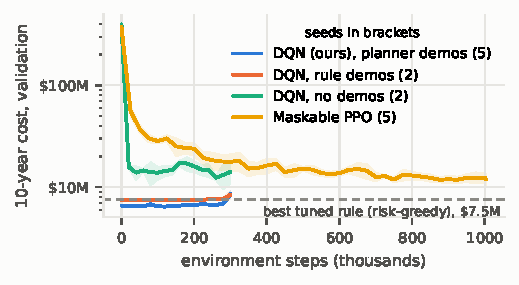
\includegraphics[width=\columnwidth]{figures/fig1_learning.pdf}
\vspace{-14pt}
\caption{Validation cost during training (mean, 95\% CI over seeds). With demonstrations, step 0 is after offline pre-training; the rise at the end is where the margin reaches zero.}
\label{fig:learning}
\end{figure}

\section{Results}
\textbf{Main result.} Over five seeds, our agent costs \$\MainCost M \mbox{[\MainLo, \MainHi]} over ten
years, \GainVsRule\% below the best tuned rule (\BestRule, \$\BestRuleCost M). The paired saving is
\$\GainVsRuleAbs M \mbox{[\GainVsRuleLo, \GainVsRuleHi]} over test episodes, and \$\MainSeedSaveRule M
\mbox{[\MainSeedSaveRuleLo, \MainSeedSaveRuleHi]} when the training seeds are resampled too. It is level with its teacher, the planner
(\$\GainVsPlanner M \mbox{[\GainVsPlannerLo, \GainVsPlannerHi]} cheaper), at \DQNms\,ms per decision
instead of \Plannerms\,ms. On as many repairs, it spends more than the rule (\$\MainAgency M vs
\$\RuleAgency M) but cuts structural risk (\$\MainRisk M vs \$\RuleRisk M) and the final restore cost
(\$\MainSalvage M vs \$\RuleSalvage M).

\textbf{What matters} (Table~\ref{tab:main}, Fig.~\ref{fig:learning}). \emph{Sharing one network across
bridges:} the flat MLP costs \$\FlatCost M, while the per-bridge variants beat the best rule unless
tied to it by rule demonstrations. The price-of-money decomposition adds nothing on top: the plain shared network with the same
demonstrations is the best agent (\$\SharedCost M, \$\SharedGap M \mbox{[\SharedGapLo, \SharedGapHi]}
cheaper than ours). \emph{A teacher is not needed:} from scratch the agent reaches \$\NoDemoCost M
(\$\NoDemoSeedSaveRule M \mbox{[\NoDemoSeedSaveRuleLo, \NoDemoSeedSaveRuleHi]} below the rule, two seeds)
and is still improving at $3{\times}10^5$ steps. \emph{Demonstrations give the final level at once:}
offline pre-training alone gives \$\PretrainCost M, and online Q-learning with the fading margin does not
improve on it; once the margin reaches zero at the very end, several seeds get worse. Rule demonstrations tie the agent to the rule (\$\RuleDemoCost M). Maskable PPO
(\$\PPOCost M) and vanilla DQN (\$\VanillaCost M) do not reach the rules.

\textbf{Value of information} (Fig.~\ref{fig:info}a). Seeing the true condition is worth \$\OracleGap M
\mbox{[\OracleGapLo, \OracleGapHi]}. Neither the belief nor paid inspections recover much of it: agents
that see only the last inspection (\$\LastObsCost M) or cannot buy inspections (\$\NoInspCost M) are
within noise of ours, because routine ratings are already accurate ($\sigma{=}\RoutineSigma$).

\textbf{Robustness} (Fig.~\ref{fig:info}b). Without retraining, the agent stays cheaper than the best rule under slower decay (+\SlowSaving), faster decay (+\FastSaving) and a 25\% funding cut
(\$\CutOurs M vs \$\CutRule M). There is no clear difference under decay faster than the model expects
(\UnmodSaving\ \mbox{[\UnmodLo, \UnmodHi]}) or noisier routine ratings
(\NoisySaving\ \mbox{[\NoisyLo, \NoisyHi]}). On twenty unseen networks of real bridges it is worse
(\$\UnseenOurs M vs \$\UnseenRule M, CI over networks \mbox{[\UnseenLo, \UnseenHi]}): it does not
transfer.


\textbf{Limitations.} One training network; two seeds per ablation; assumed unit and risk costs.

\end{document}
